\documentclass[12pt,a4paper]{article}
\usepackage[russian]{babel}
\usepackage[cp1251]{inputenc}
\usepackage{amsmath,amssymb}
\usepackage{graphicx}
\usepackage{cite}
\usepackage{wrapfig}
\usepackage{physics}
\usepackage{wrapft}
\usepackage{epstopdf}
\usepackage[small]{caption}
\usepackage{subcaption}

\renewcommand{\baselinestretch}{1.0}

\usepackage{indentfirst} % отделять первую строку раздела абзацным отступом тоже
\usepackage{makecell} % фиксированный размер ячейки таблицы
\usepackage{multirow} % улучшенное форматирование таблиц, объединение строк

\usepackage{enumitem}

\oddsidemargin	-1cm
\topmargin		-2cm
\textwidth		18.2cm
\textheight		24.2cm

\newcommand{\D}{\displaystyle}


\righthyphenmin=0
\parindent=0mm
\parskip= 2.0 mm
\righthyphenmin=0



\begin{document}
	
	\graphicspath{{figures/}}
	
	\baselineskip = 20 true pt \vspace{40mm} \large
	\begin{titlepage}
		\begin{center}
			Федеральное государственное бюджетное образовательное учреждение высшего образования\\[0.5cm]
			Омский государственный университет им. Ф.М. Достоевского\\[4.5cm]
			
			Математическое моделирование\\ уравнений математической физики\\[2cm]
			Задание № 1\\[1cm]
			\uppercase{{\large{
						Численные методы решения задачи Коши для системы обыкновенных дифференциальных уравнений
			}}}\\[3cm]
			Вариант №\ 8 - 6\\[2cm]
		\end{center}
		
		\begin{flushright}
			Выполнил:\\
			студент группы ФПБ-803\\
			Хитринцевва Валерия Вадимовна\\[3cm]
		\end{flushright}
		
		\begin{center}
			Омск-2021
		\end{center}
	\end{titlepage}
	
	%>>>>>>>>>>>>>>>>>>>>>>>>>>>>>>>>>>>>>>>>>>>>>>>>>>>>>>>>>>>>>>>>>>>>>>>>>>>>>>>>>>>>>>>>>>>>>>>>>>>>>>>
	\setcounter{page}{2} 
	\tableofcontents
	\newpage
	%>>>>>>>>>>>>>>>>>>>>>>>>>>>>>>>>>>>>>>>>>>>>>>>>>>>>>>>>>>>>>>>>>>>>>>>>>>>>>>>>>>>>>>>>>>>>>>>>>>>>>>>
	
	%>>>>>>>>>>>>>>>>>>>>>>>>>>>>>>>>>>>>>>>>>>>>>>>>>>>>>>>>>>>>>>>>>>>>>>>>>>>>>>>>>>>>>>>>>>>>>>>>>>>>>>>
	\newpage
	\section{Постановка задачи}
	\begin{enumerate}[itemindent=0.0em]
		\setlength{\itemsep}{1pt}%
		\item Разработать программу для ЭВМ решения краевой задачи для уравнения теплопроводности, реализующую предложенный численный метод и дополнительные вычислительные процедуры. Численное решение задачи осуществить с использованием методом прямых, с дискретизацией по пространственным переменным. 
		
		\item  С использованием разработанной программы для ЭВМ осуществить решение тестовой краевой задачи
		для уравнения теплопроводности для теплофизически однородного материала без внутренних источников.
		\item С использованием разработанной программы для ЭВМ осуществить решение индивидуального задания	с краевой задачи для уравнения теплопроводности. Построить зависимости решения $u = u(r, t)$ от координат
		$r$ для нескольких значений временной переменной $t$: в случае двумерной задачи требуется построить
		двумерные зависимости решения $u(r, t)$ от координат $r = (x, y)$. 
	\end{enumerate}
	
	Для выполнения данного задания требуется реализовать метод прямых. Основная идея метода прямых состоит в сведении уравнений в частных производных к решению системы обыкновенных дифференциальных уравнений. Метод прямых может быть использован для решения уравнений в частных производных любого типа, но используется в основном для решения эллиптических и параболических уравнений.
	Уравнение теплопроводности задается в виде
	\begin{equation}
		c(\textbf{r}) \displaystyle \frac{\partial u}{\partial t} = \displaystyle \frac{\partial}{\partial \textbf{r}} \biggl( \lambda(\textbf{r}) \displaystyle \frac{\partial u}{\partial \textbf{r}}\biggl) + f(\textbf{r}, t) ,
	\end{equation}
	где $u = u(\textbf{r}, t)$ — искомая функция, зависящая от координаты $r$ и времени $t$; $\displaystyle \frac{\partial }{\partial \textbf{r}} \equiv \Delta$ — градиент; $c = c(r)$
	и $\lambda = \lambda (\textbf{r})$ — заданные функции, определяющие пространственные зависимости удельной теплоемкости
	и коэффициента теплопроводности; $f = f(\textbf{r}, t)$ — заданная функция плотности источника.
	\\
	Для двумерного уравнения: $\textbf{r} = (x, y), \ \displaystyle  \frac{\partial }{\partial \textbf{r}} = \biggl(\frac{\partial }{\partial x},\  \frac{\partial }{\partial y} \biggl)$.\\
	Область определения решения:
	\begin{center}
		\begin{tabular}{c c c }
			$	t \geq 0 $&
			$	0 \leq x \leq L_x $&
			$	0 \leq y \leq L_y$
		\end{tabular}
	\end{center}
	
	Начальные условия задаются в видe:\begin{center}$u(\textbf{r}, t = 0) = \phi (\textbf{r});$\end{center}
	В данной работе рассматриваются граничные условия в виде первой краевой задачи по $x$ и второй краевой задачи по $y$:
	\begin{center}
		\begin{tabular}{c c}
			$u(x = 0, t) = \mu_L (t)$&$ u(x = L, t) = \mu_R (t)$ \\
			$\displaystyle \frac{\partial u }{\partial y}(y = 0, t) = \mu_L (t)$&$\displaystyle \frac{\partial u }{\partial y} (y = L, t) = \mu_R (t)$
		\end{tabular}
	\end{center}
	
	
	
	Индивидуальное задание:
	\begin{center}
		\begin{tabular}{l}
			$\lambda (x, y) = 1 + \frac{1}{2} xy(1 - xy)$\\
			$c(x, y) = 1 - \frac{1}{2} \sin(\pi x) \sin(\pi y)$ \\
			$f( x, y; t) = 40 \sin(\pi x) \sin( \pi y) \th(t)$\\
			$\phi( x, y) =  \cos(2\pi x) \cos(2 \pi y) $
		\end{tabular}
	\end{center}
	
	Область определения решения:
	\begin{center}
		\begin{tabular}{c c c }
			$	t \geq 0 $&
			$	0 \leq x \leq 1 $&
			$	0 \leq y \leq 1$
		\end{tabular}
	\end{center}
	Граничные условия:
	\begin{center}
		\begin{tabular}{c c }
			$u(x = 0, y, t) = \mu_L (y, t)$& $\mu_L (y, t) = \cos(2\pi y)$\\
			$u(x = 1, y, t) = \mu_R (y, t)$& $\mu_R (y, t) = \cos(2\pi y)$\\
			$\  \frac{\partial u }{\partial y} (x, y = 0, t) = \mu_B (x, t)$ &$\mu_B (x, t) = 0$\\
			$\  \frac{\partial u }{\partial y} (x, y = 1, t) = \mu_T (x, t)$ &$\mu_T (x, t) = 0$\\
		\end{tabular}
	\end{center}
	
	
	
	Индивидуальное задание:
	\begin{center}
		\begin{tabular}{l}
			$\lambda (x, y) = 1 + \frac{1}{2} xy(1 - xy)$\\
			$c(x, y) = 1 - \frac{1}{2} \sin(2 \pi x) \sin(2 \pi y)$ \\
			$f( x, y; t) = 40\ x^4 y^4 (1 - x^4 y^4) \th(\frac{t}{10})$\\
			$\phi( x, y) =  \cos(4\pi x) \cos(4 \pi y) $
		\end{tabular}
	\end{center}
	
	Область определения решения:
	\begin{center}
		\begin{tabular}{c c c }
			$	t \geq 0 $&
			$	0 \leq x \leq 1 $&
			$	0 \leq y \leq 1$
		\end{tabular}
	\end{center}
	Граничные условия:
	\begin{center}
		\begin{tabular}{c c }
			$u(x = 0, y, t) = \mu_L (y, t)$& $\mu_L (y, t) = \cos(4\pi y)$\\
			$u(x = 1, y, t) = \mu_R (y, t)$& $\mu_R (y, t) = \cos(4\pi y)$\\
			$\  \frac{\partial u }{\partial y} (x, y = 0, t) = \mu_B (x, t)$ &$\mu_B (x, t) = 0$\\
			$\  \frac{\partial u }{\partial y} (x, y = 1, t) = \mu_T (x, t)$ &$\mu_T (x, t) = 0$\\
		\end{tabular}
	\end{center}
	
	
	%>>>>>>>>>>>>>>>>>>>>>>>>>>>>>>>>>>>>>>>>>>>>>>>>>>>>>>>>>>>>>>>>>>>>>>>>>>>>>>>>>>>>>>>>>>>>>>>>>>>>>>>
	\newpage
	\section{Полученные результаты и их анализ}
	\numberwithin{figure}{subsection}
	Для всех приведенных далее результатов использовались следующие параметры моделирования:
	\begin{enumerate}
		\item Область определения: $L_x = 1.0, \ L_y = 1.0.$
		\item Количество узлов сетки: $N_x = N_y = 100.$
		\item Временной диапазон $t \in [0.0, 5.0]$.\\ Шаг по времени $\tau$ определяется по формуле $\tau = 0.5 CFL$, где $CFL \leq 1$ -- условие Куранта, Фридрихса, Леви. $h$ -- шаг по сетке
	\end{enumerate}
	\subsection{Решение тестовых задач}
	\begin{figure}[h!]
		\begin{minipage}[h]{0.5\linewidth}
			\centering{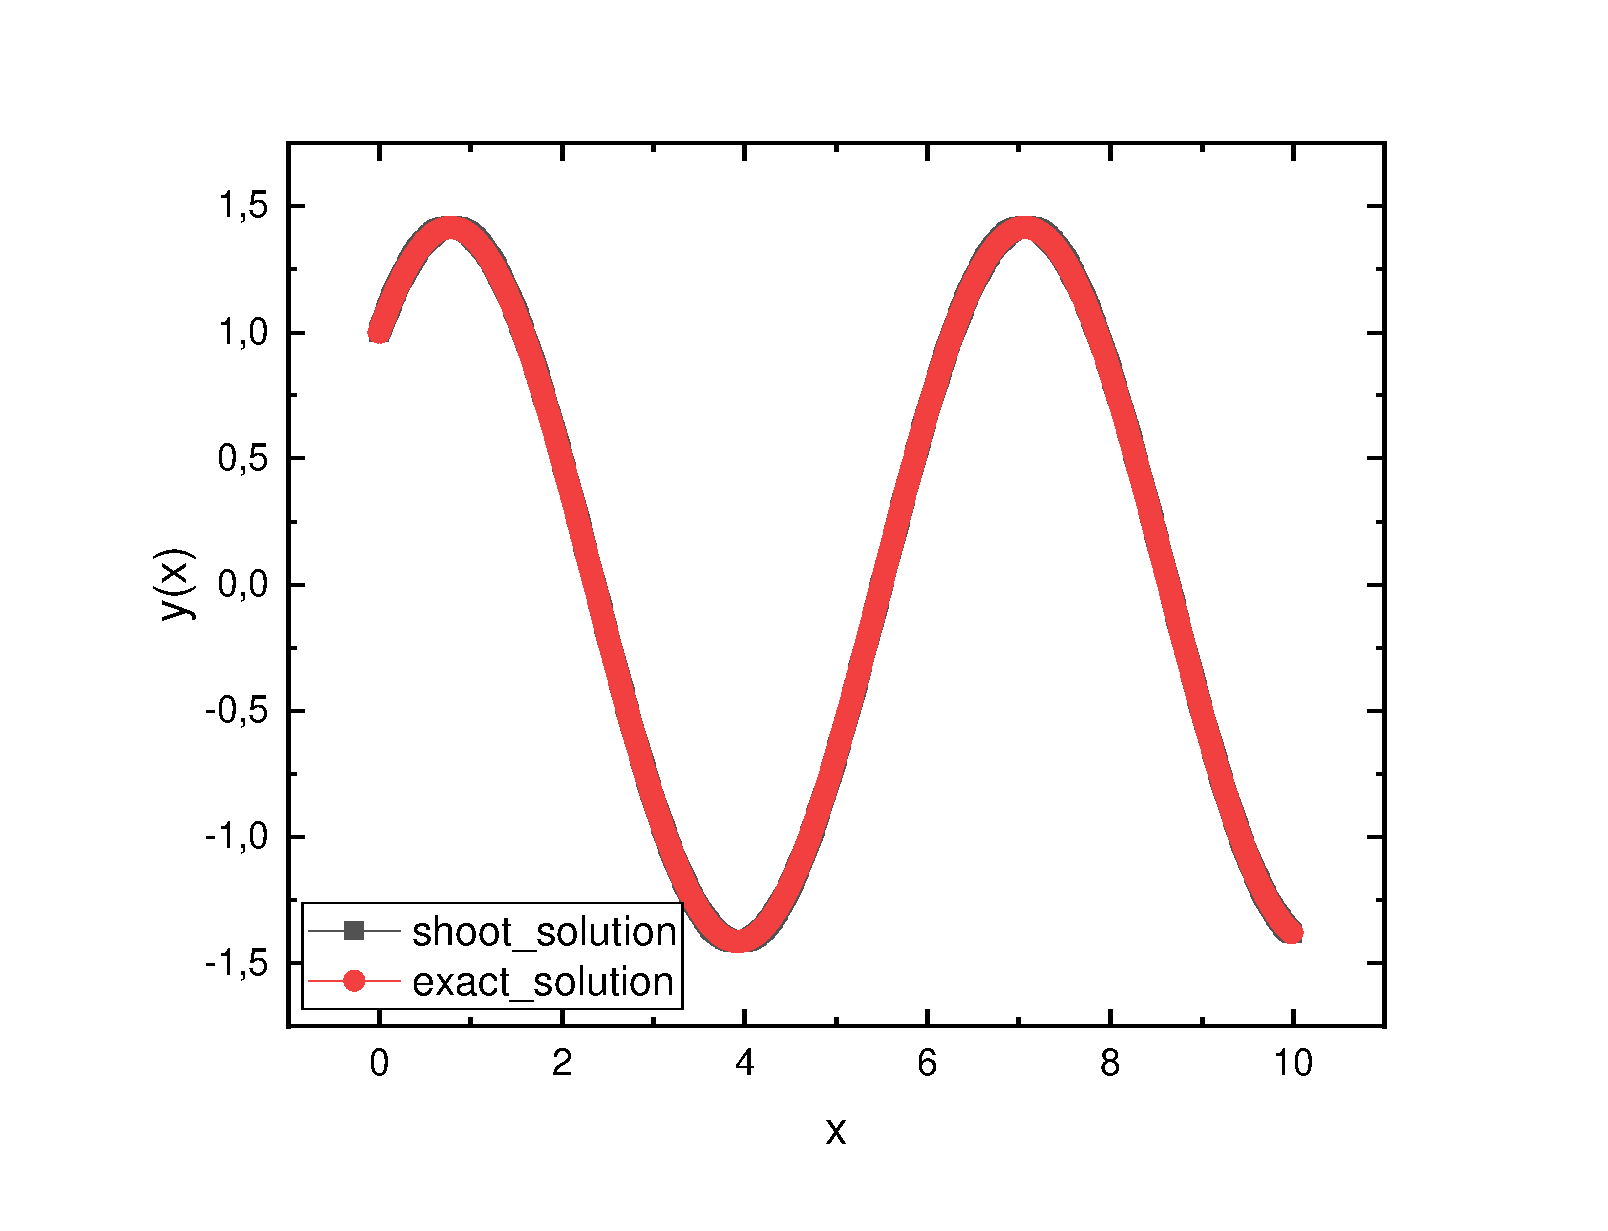
\includegraphics[width=\textwidth]{graph_2/first_pr.pdf} а)}
		\end{minipage}
		\begin{minipage}[h]{0.5\linewidth}
			\centering{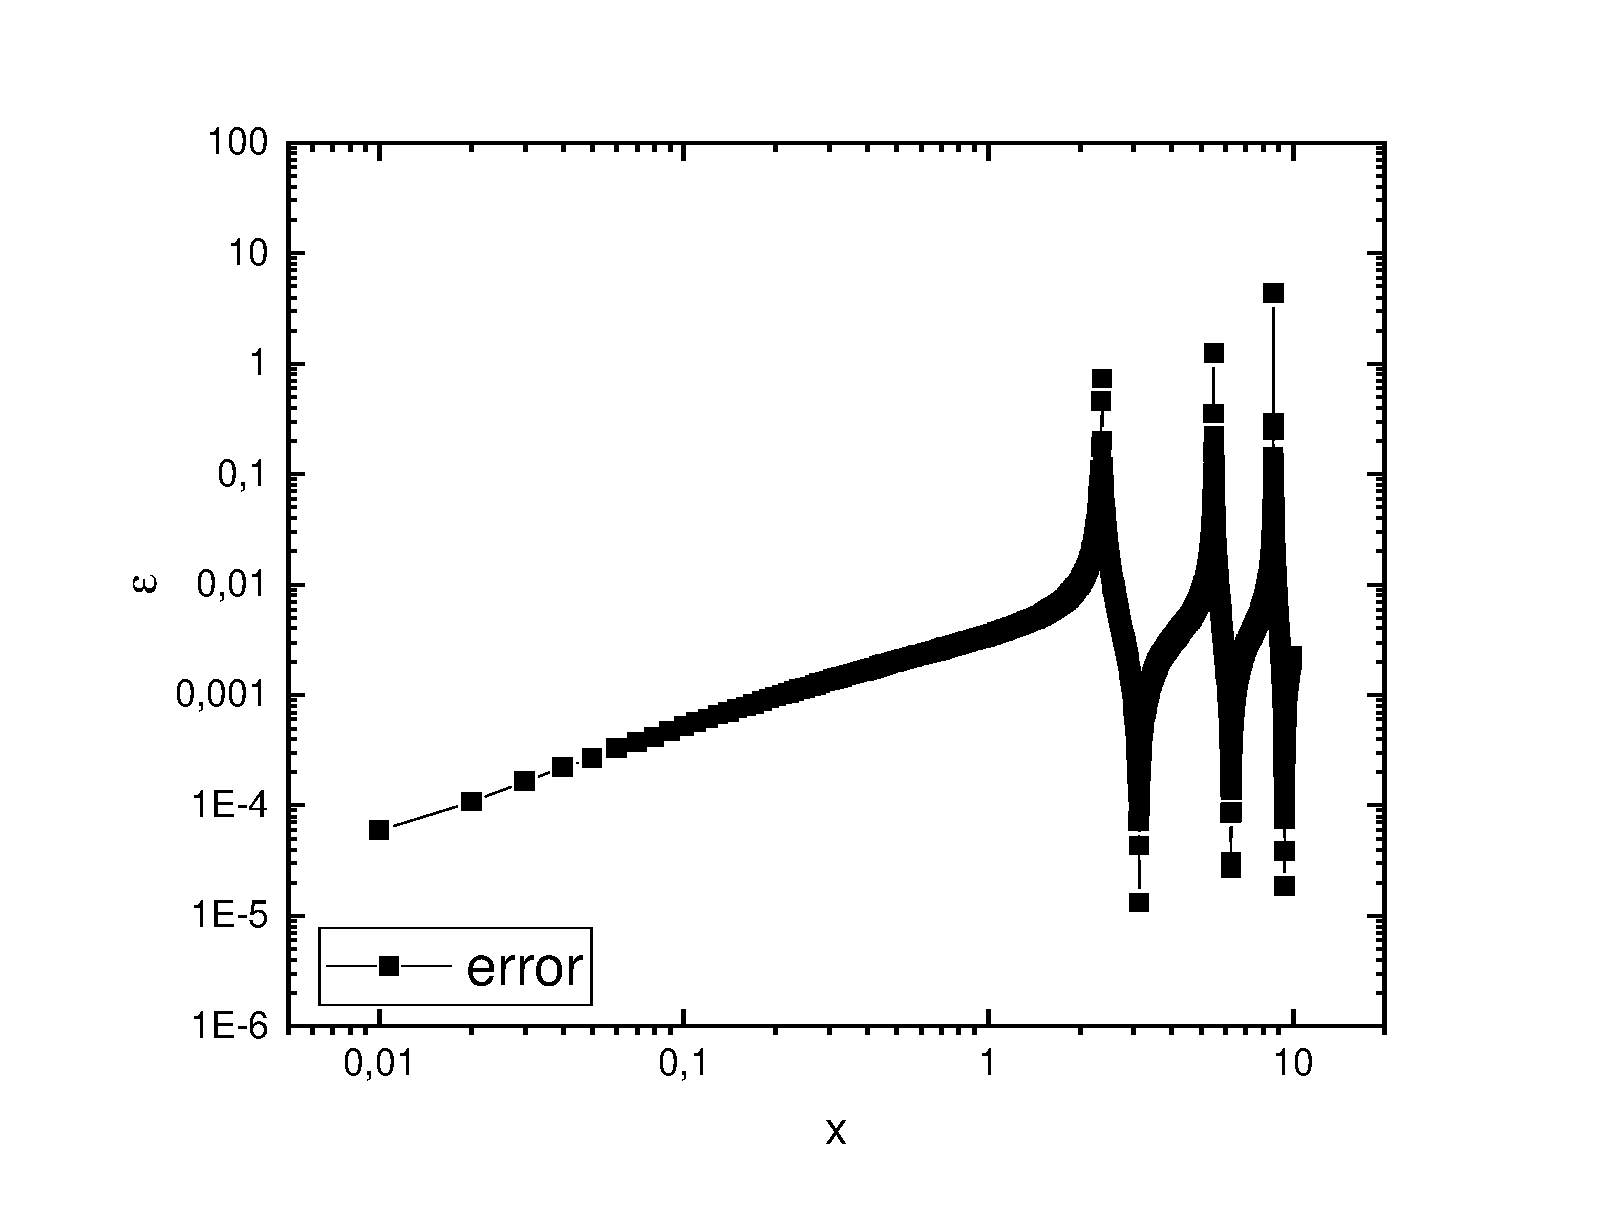
\includegraphics[width=\textwidth]{graph_2/error_first.pdf} б)}
		\end{minipage}
		\begin{minipage}[h]{0.5\linewidth}
			\centering{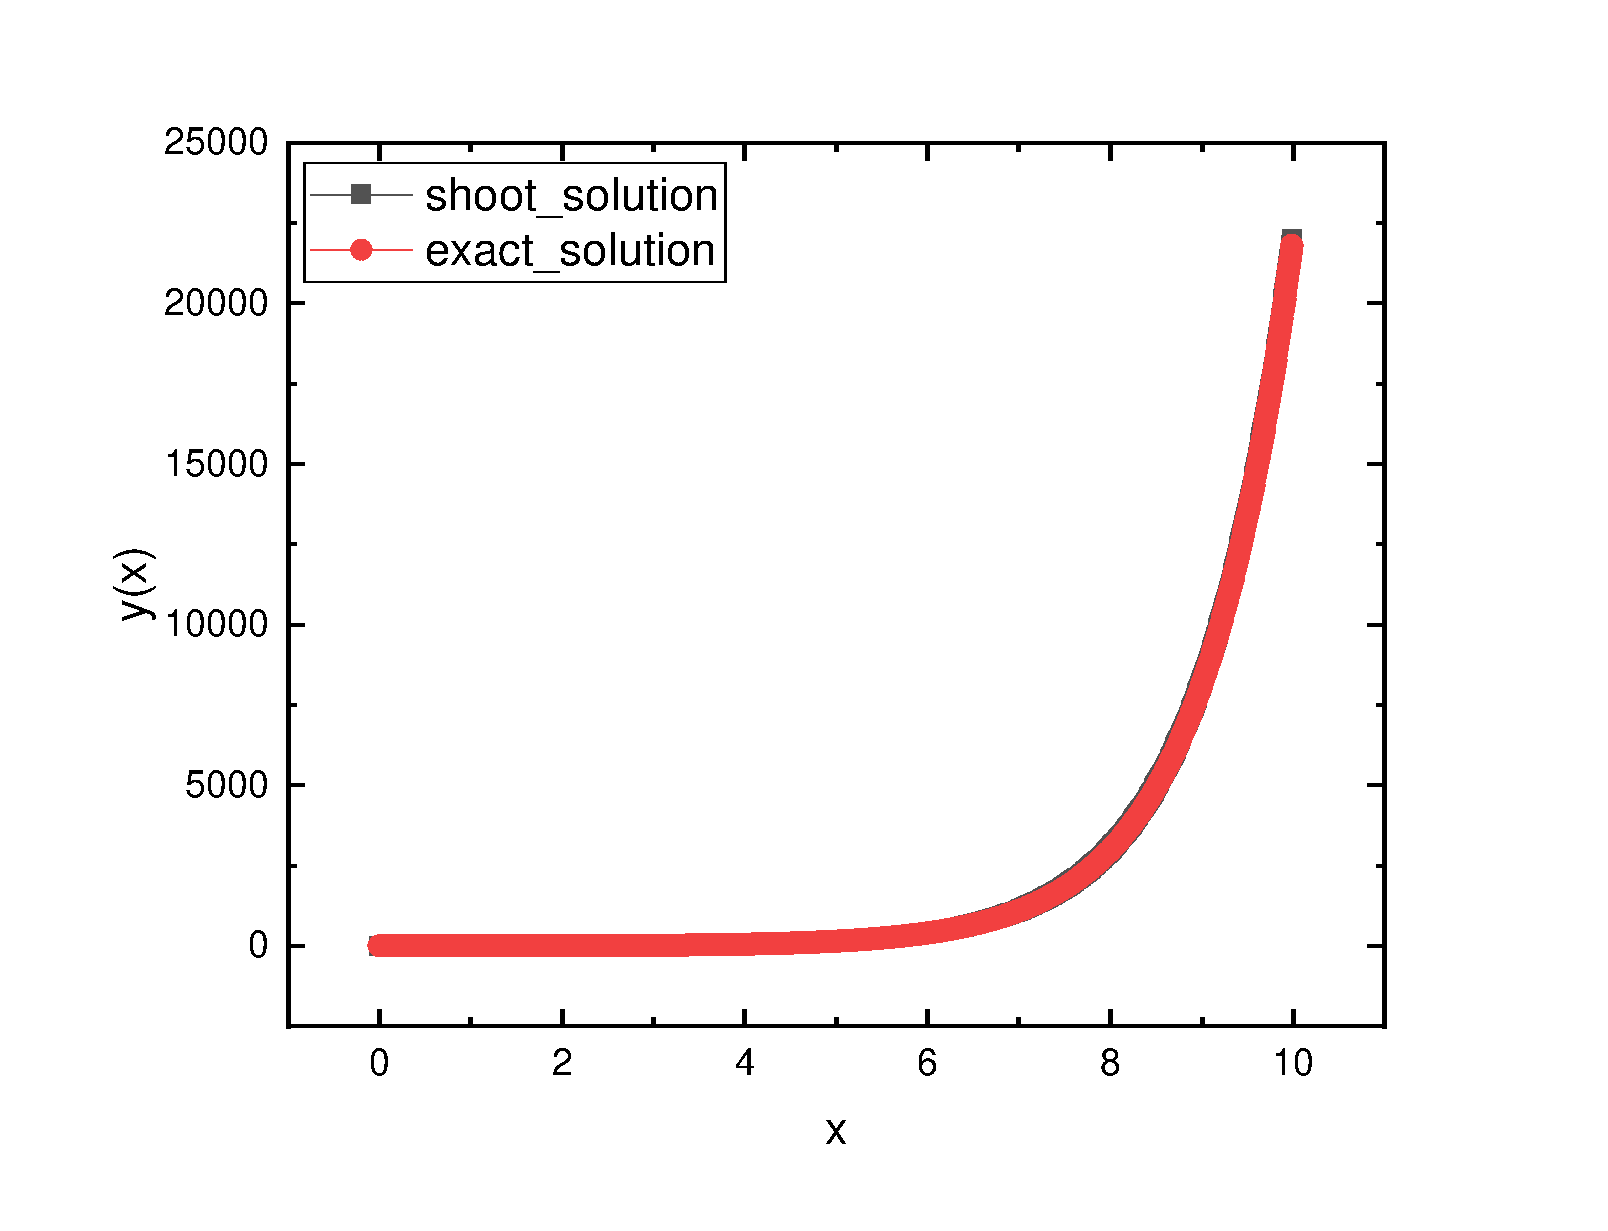
\includegraphics[width=\textwidth]{graph_2/second_pr.pdf} в)}
		\end{minipage}
		\begin{minipage}[h]{0.5\linewidth}
			\centering{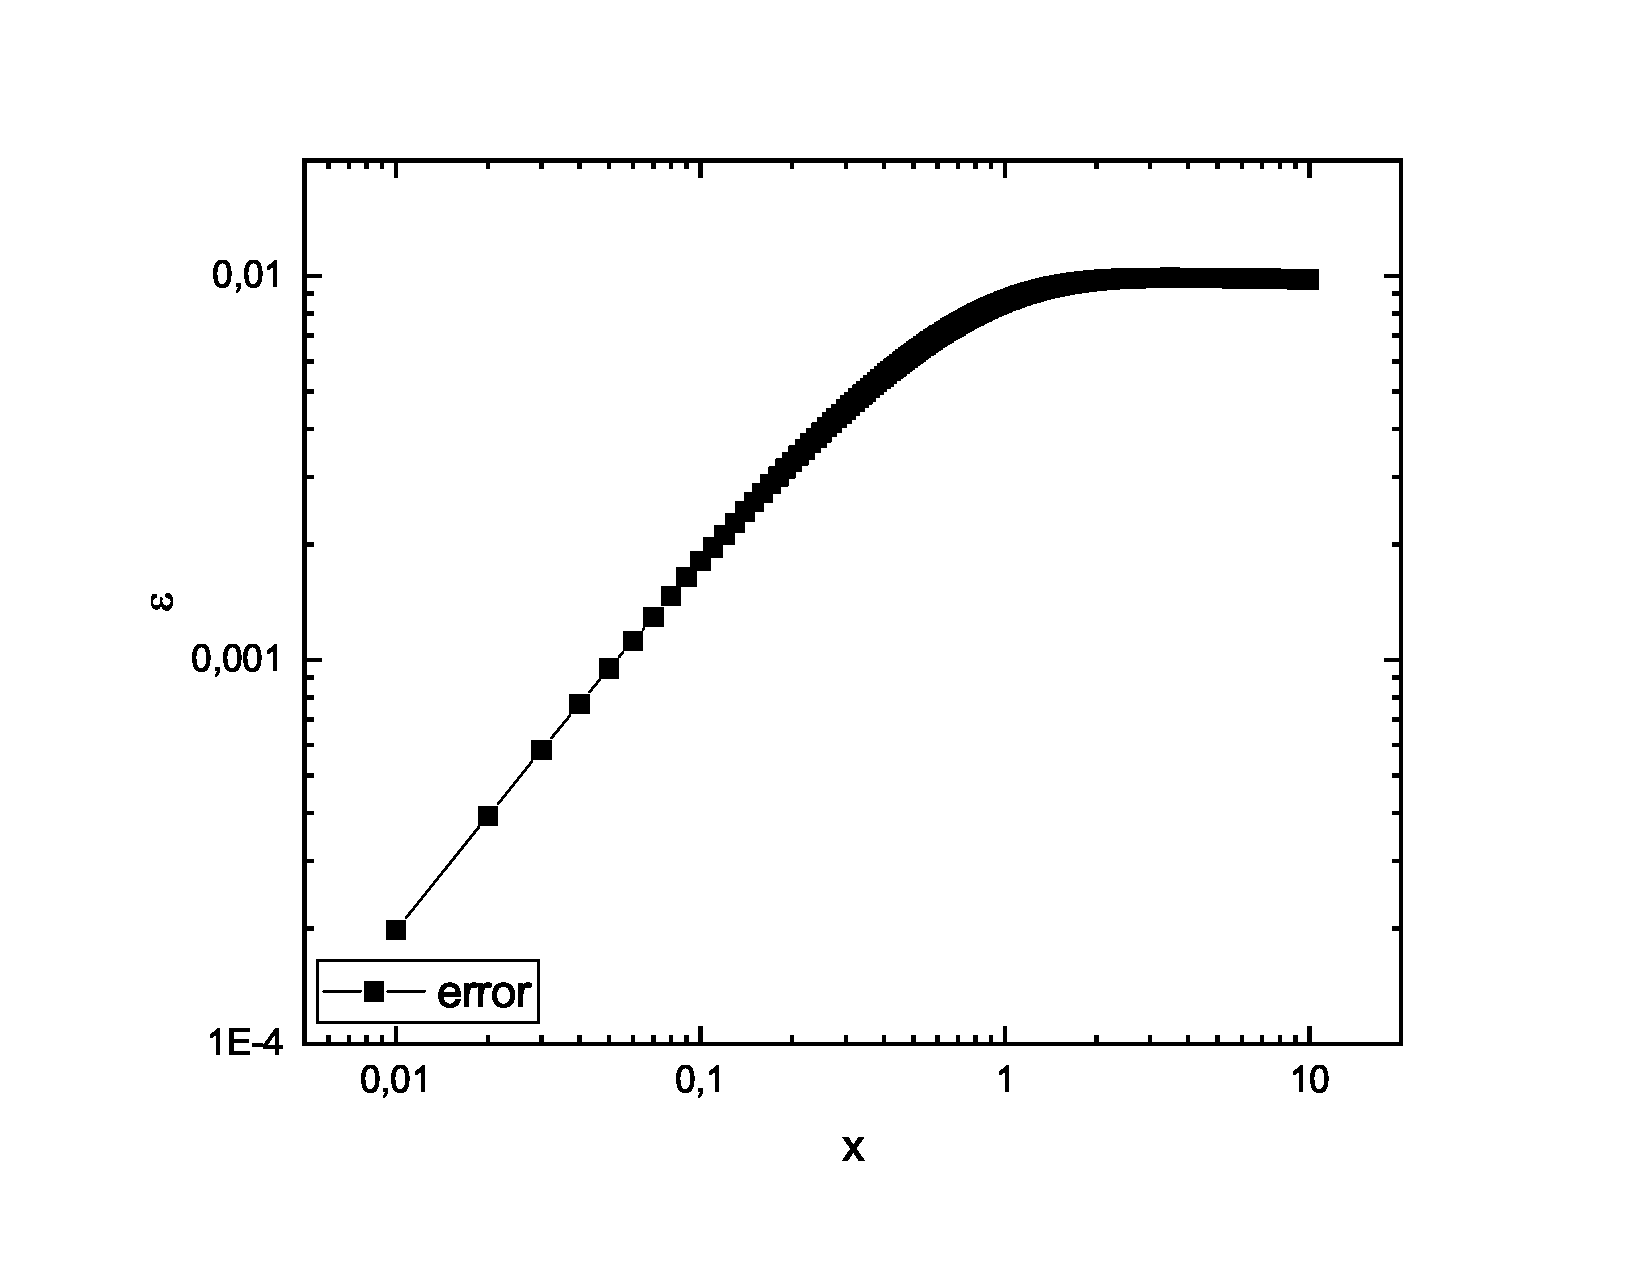
\includegraphics[width=\textwidth]{graph_2/second_error.eps} г)}
		\end{minipage}
		\begin{minipage}[h]{0.5\linewidth}
			\centering{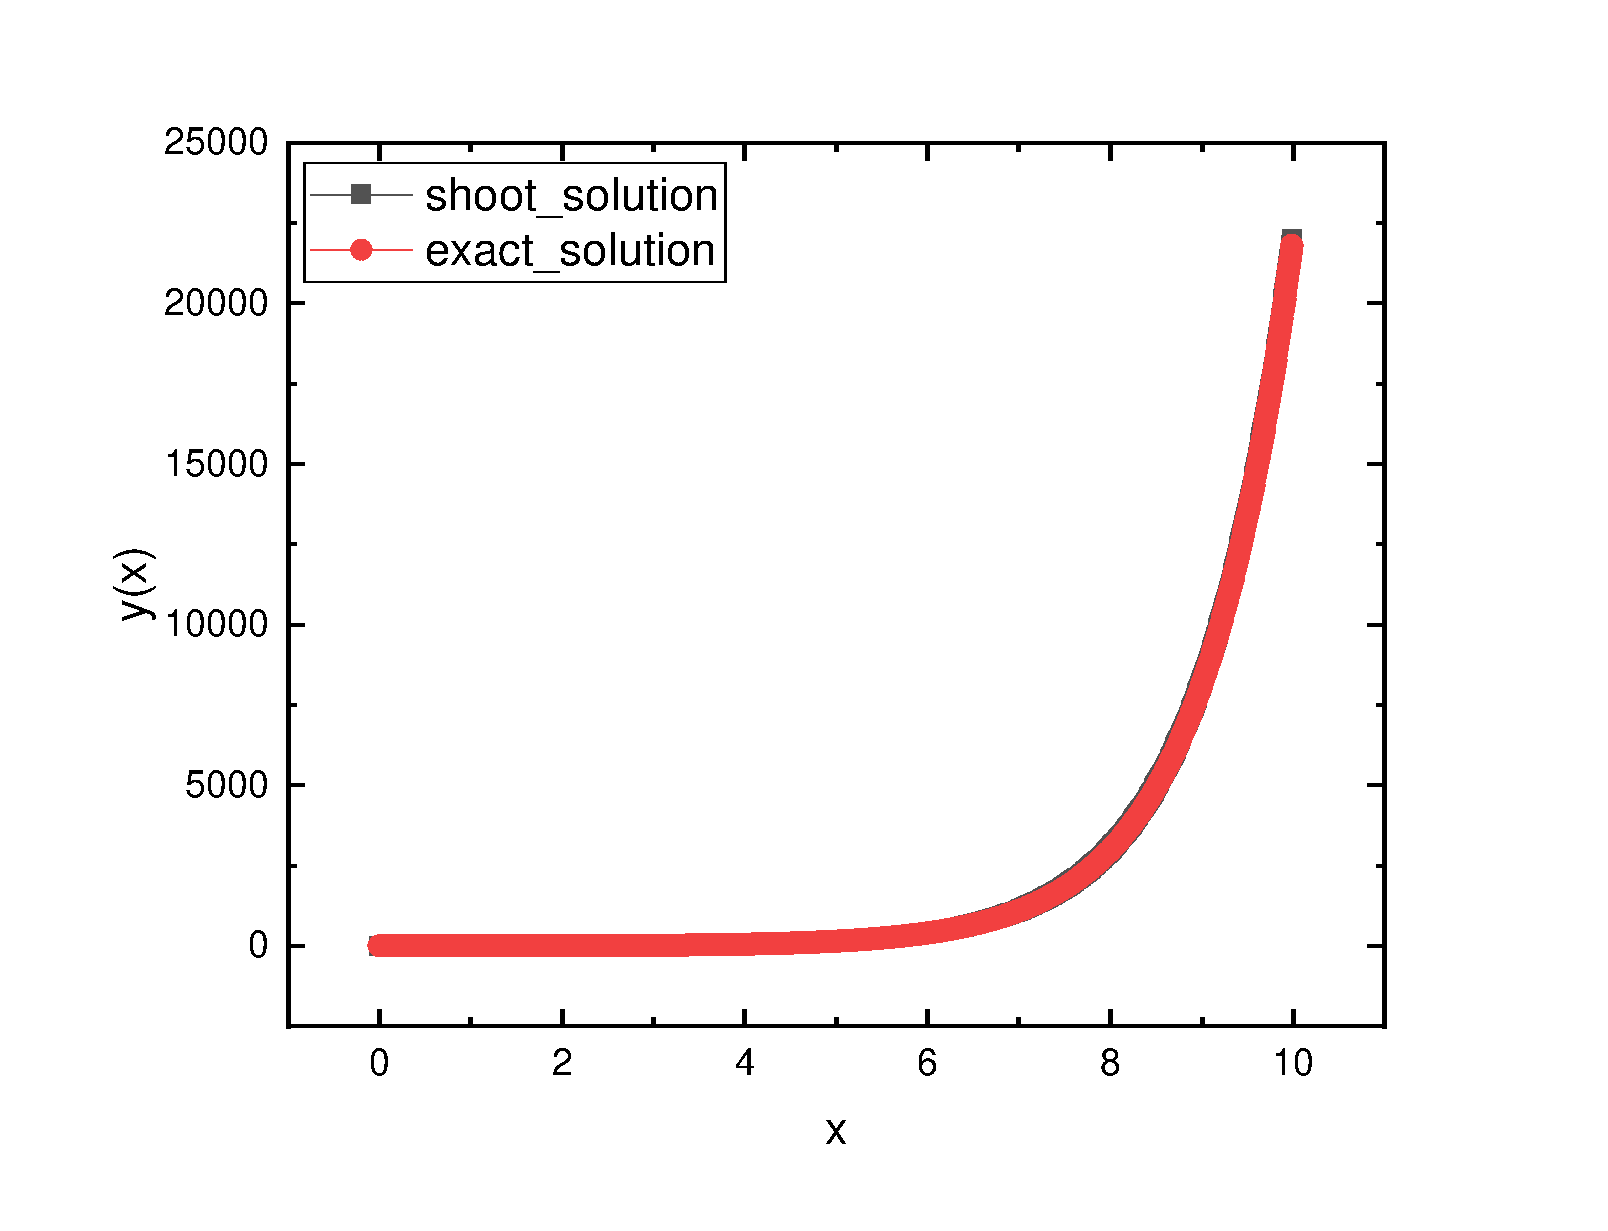
\includegraphics[width=\textwidth]{graph_2/second_pr.pdf} в)}
		\end{minipage}
		\begin{minipage}[h]{0.5\linewidth}
			\centering{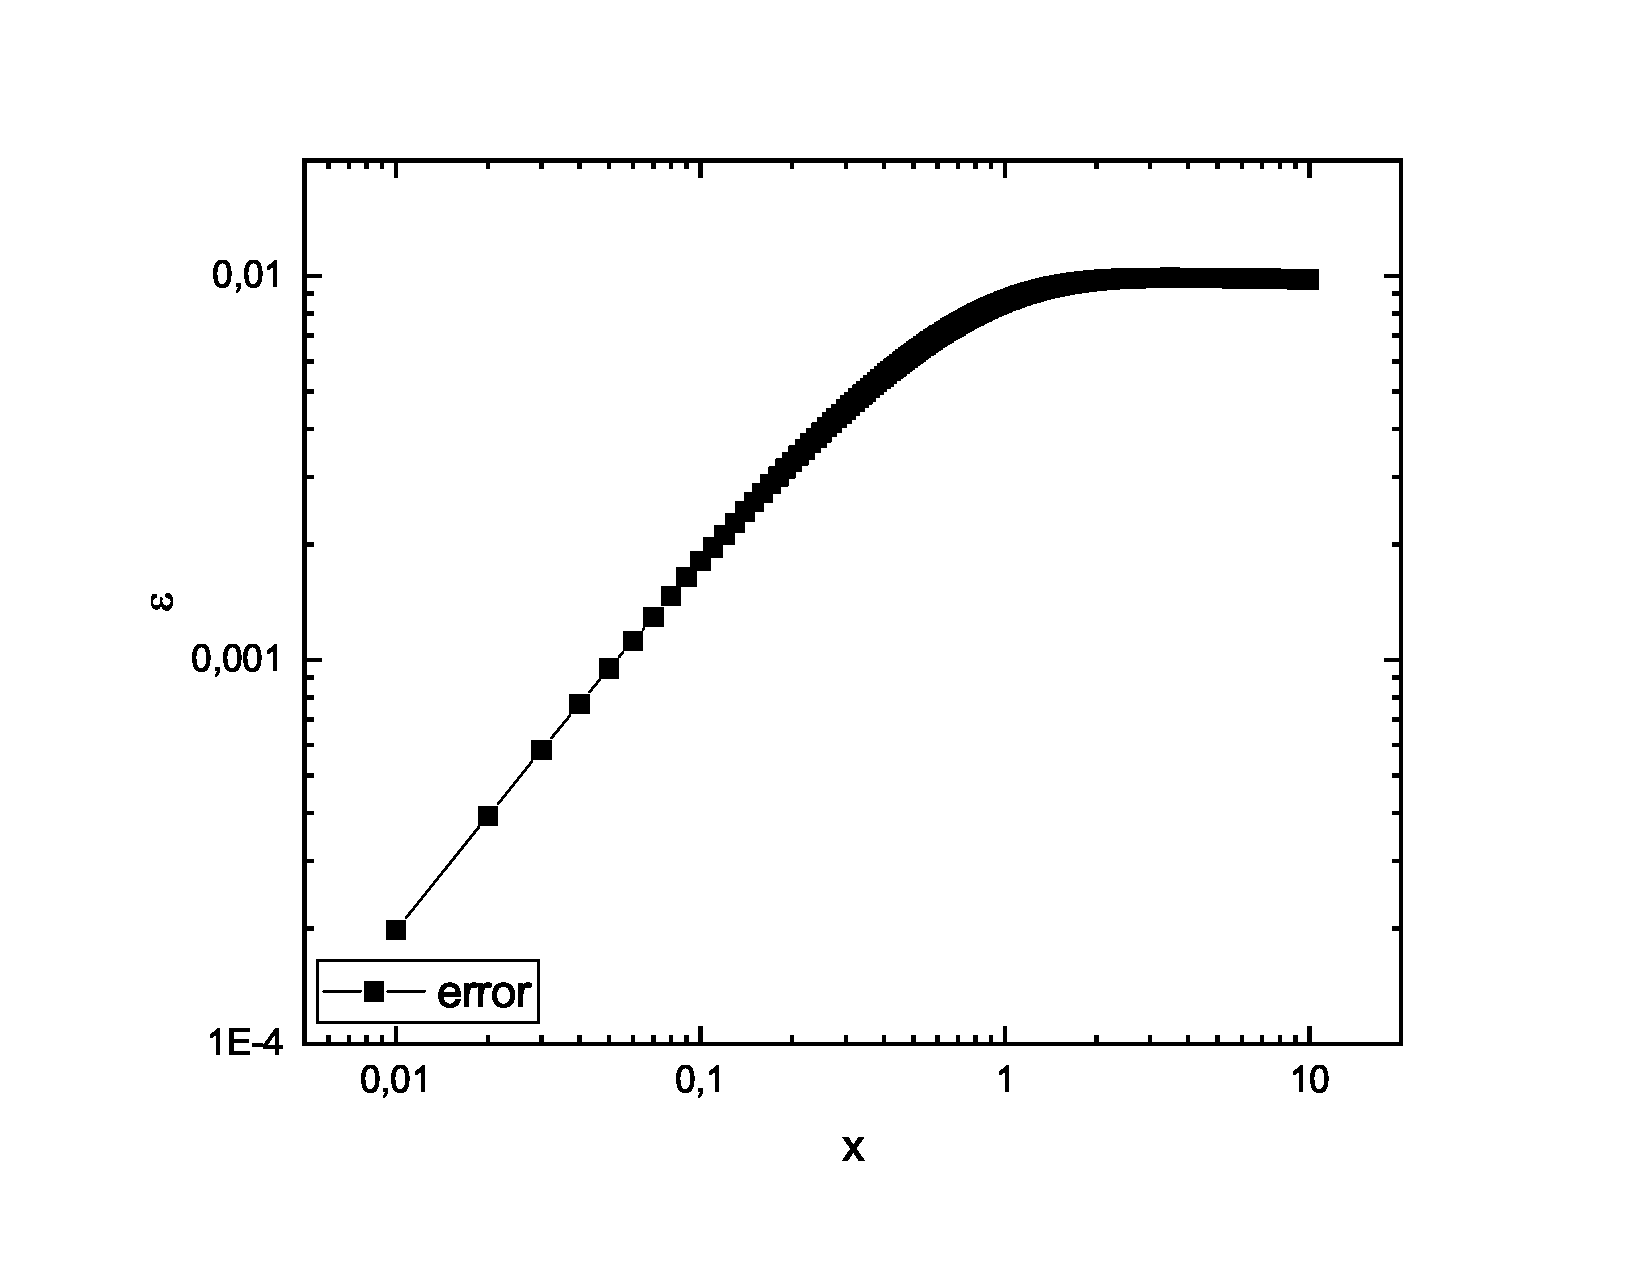
\includegraphics[width=\textwidth]{graph_2/second_error.eps} г)}
		\end{minipage}
		\caption{Зависимость решения $y = y(x)$ и погрешность вычислений для a), б) - первый тестовой задачи, в), г) - второй тестовой задачи}
	\end{figure}
	\par Анализируя полученные графики, можно отметить, что решение, полученное методом пристрелки, соответствует точному решению.
	
	
	
	
	%>>>>>>>>>>>>>>>>>>>>>>>>>>>>>>>>>>>>>>>>>>>>>>>>>>>>>>>>>>>>>>>>>>>>>>>>>>>>>>>>>>>>>>>>>>>>>>>>>>>>>>>
	\newpage
	\section*{Заключение}
	\addcontentsline{toc}{section}{Заключение} \hspace*{1cm}
	В данной работе были рассмотрены:
	\begin{enumerate}
		\item Тестовая краевая задача. Построены зависимости $u(x) = u(\textbf{r} , t)$, построены срезы.
		\item Индивидуальная задача. Получено решение индивидуального задания с краевой задачей для уравнения теплопроводности $(2 - 13)$.
		Построены зависимости решения $u = u(r, t)$ от координат $r$ для нескольких значений временной зависимости $t$.
	\end{enumerate}
	Для решения граничной задачи был реализован метод прямых. Задача Коши решается многошаговым методом Адамса-Мултона со стартовым методом Лобатто $IIIC$ второго порядка точности.\\
	
	
	%>>>>>>>>>>>>>>>>>>>>>>>>>>>>>>>>>>>>>>>>>>>>>>>>>>>>>>>>>>>>>>>>>>>>>>>>>>>>>>>>>>>>>>>>>>>>>>>>>>>>>>>
	
	\newpage
	\addcontentsline{toc}{section}{Список литературы}
	\begin{thebibliography}{99}
		
		\bibitem{Kalitkin_2013_1}
		Калиткин Н.Н., Альшина Е.А., Корякин П.В. 
		Численные методы. Книга 1. Численный анализ. --- М.: Академия, 2013. 
		
		\bibitem{Kalitkin_2013_2}
		Калиткин Н.Н., Корякин П.В. 
		Численные методы. Книга 2. Методы математической физики. --- М.: Академия, 2013. 
		
		\bibitem{Kalitkin_BJK_2003}
		Бахвалов Н.С., Жидков Н.П., Кобельков Г.М. 
		Численные методы. --- М.: Бином, 2003, 2012.
		
		\bibitem{HNW_I}
		Хайрер Э., Нёрсетт С., Ваннер Г. 
		Решение обыкновенных дифференциальных уравнений. 
		Нежесткие задачи. --- М.: Мир, 1990.
		
		\bibitem{HNW_II}
		Хайрер Э., Ваннер Г. 
		Решение обыкновенных дифференциальных уравнений. 
		Жесткие и дифференциально-алгебраические задачи. --- М.: Мир, 1999.
		
		\bibitem{Butcher_2016}
		Butcher J.C. Numerical Methods for Ordinary Differential Equations. --- 
		John Wiley \& Sons, 2016.
		
	\end{thebibliography}
\end{document}
